\documentclass[compress]{beamer}
\usecolortheme{default}

\usepackage{lmodern, epstopdf, multirow, array, setspace, bbm, tcolorbox, pbox, bm, mathtools, tikz}
\usepackage[T1]{fontenc}

\setbeamertemplate{frametitle}[default][center]
\setbeamertemplate{footline}{\hfill \insertframenumber/\inserttotalframenumber\hspace*{5pt}\vspace{5pt}}
\setbeamertemplate{navigation symbols}{}

\newlength{\wideitemsep}
\setlength{\wideitemsep}{\itemsep}
\addtolength{\wideitemsep}{4pt}
\let\olditem\item
\renewcommand{\item}{\setlength{\itemsep}{\wideitemsep}\olditem}
\setlength{\leftmargini}{12pt}
\setlength{\leftmarginii}{14pt}
\setbeamertemplate{itemize/enumerate subbody begin}{\vspace{6pt}}
\setbeamertemplate{itemize item}[circle]
\setbeamertemplate{enumerate item}[circle]
\setbeamertemplate{enumerate subitem}[default]

\setbeamercolor{alerted text}{fg=blue}
\setbeamersize{text margin left=1.5em,text margin right=1.5em}

\tcbset{
    colback=white,
    colframe=black,
    coltext=black,
    coltitle=blue,
    colbacktitle=white,
    boxrule=1pt,
    titlerule=0pt,
    toptitle=4pt,
    top=2pt
}

\newenvironment{changemargin}[2]{% 
  \begin{list}{}{% 
    \setlength{\topsep}{0pt}% 
    \setlength{\leftmargin}{#1}% 
    \setlength{\rightmargin}{#2}% 
    \setlength{\listparindent}{\parindent}% 
    \setlength{\itemindent}{\parindent}% 
    \setlength{\parsep}{\parskip}% 
  }% 
  \item[]}{\end{list}}
  
\newenvironment{defn}{%
  \begin{tcolorbox}[title={Definition}]%
  }{\end{tcolorbox}}
  
\newenvironment{prop}[1]{%
  \begin{tcolorbox}[title={Proposition #1}]%
  }{\end{tcolorbox}}
  
\newcommand{\cit}[1]{{\footnotesize \textcolor[rgb]{0.5,0,0}{#1}}}

% Font size for code listings (verbatim blocks); reset with \normalsize
\newcommand{\codesize}{\fontsize{7}{8.5}\selectfont}

\newcommand{\slidesetup}[1]{%
  \title{#1}%
  \subtitle{\texorpdfstring{\vspace{0.3\baselineskip}}{} {\small This version: \today}}%
  \author[Mikkel Plagborg-Moller]{ECMA 31150, Spring 2026 \texorpdfstring{\\[0.5ex]}{} University of Chicago \texorpdfstring{\\[0.5ex]}{} Department of Economics \texorpdfstring{\\[4ex]}{} Mikkel Plagborg-Moller}%
  \date{}%
}

% \circleoverlay[options]{text}
% Draws a red circle with a text box nearby on a tikz overlay.
% Options (with defaults):
%   cx=0cm, cy=0cm      - circle center (shift from page center)
%   r=1cm               - circle radius
%   tx=0cm, ty=0cm      - text box offset from circle center
%   text anchor=east    - anchor of text node (east = text left, west = text right)
%   font=\normalsize    - font size for text
\pgfkeys{
  /circleoverlay/.cd,
  cx/.store in=\cocx, cx=0cm,
  cy/.store in=\cocy, cy=0cm,
  r/.store in=\cor, r=1cm,
  tx/.store in=\cotx, tx=0cm,
  ty/.store in=\coty, ty=0cm,
  text anchor/.store in=\cotextanchor, text anchor=east,
  font/.store in=\cofont, font=\normalsize,
}
\newcommand{\circleoverlay}[2][]{%
  \pgfkeys{/circleoverlay/.cd, cx=0cm, cy=0cm, r=1cm, tx=0cm, ty=0cm, text anchor=east, font=\normalsize, #1}%
  \pgfmathsetlengthmacro{\circlediameter}{2*\cor}%
  \node[draw=red, line width=2pt, circle, minimum size=\circlediameter, inner sep=0pt]
    (tmpcirc) at ([xshift=\cocx,yshift=\cocy]current page.center) {};%
  \node[anchor=\cotextanchor, fill=white, draw=red, text=red, inner sep=4pt, align=left, font=\cofont]
    at ([xshift=\cotx,yshift=\coty]tmpcirc.center) {#2};%
}

\DeclareMathOperator*{\argmax}{argmax}
\DeclareMathOperator*{\argmin}{argmin}
\DeclareMathOperator{\diag}{diag}
\DeclareMathOperator{\var}{Var}
\DeclareMathOperator{\cov}{Cov}
\DeclareMathOperator{\corr}{Corr}
\DeclareMathOperator{\lrv}{LRV}


\slidesetup{Bayesian estimation I}

\begin{document}
\frame{
\maketitle
}

\frame{
\frametitle{Plan for this slide deck}
\begin{enumerate}
\item Bayesian inference: using prior knowledge to inform estimation
\item Computational techniques
\item Bayesian software: Stan
\end{enumerate}
}

\frame{
\frametitle{Frequentist vs.\ Bayesian inference}
\begin{itemize}
\item So far in this course we have conducted \textbf{frequentist inference}: we sought statistical procedures that worked well \emph{across repeated (hypothetical) histories of the world}, regardless of what the true model parameters are.
\item \textbf{Bayesian inference} instead prioritizes some parameter values over others and seeks optimal statistical procedures given the \emph{actually observed history of the world}.
\item Before the data analysis, a Bayesian decides which parameter values to prioritize by selecting a \textbf{prior distribution} over the param.\ space.
\item The prior can be used to incorporate additional scientific knowledge that the researcher possesses before seeing the data.
\begin{itemize}
\item This can be used to \textbf{shrink} the frequentist's parameter estimates toward values that are \emph{a priori} more ``reasonable''.
\end{itemize}
\end{itemize}
}

\frame{
\frametitle{Bayesian inference}
\begin{itemize}
\item One could teach a whole course on Bayesian statistics.
\item Bayesian methods have deep methodological underpinnings that can be formalized based on decision theory (essentially, the same stuff you learn in Econ Micro Theory 101).
\item However, I will just tell you the bare minimum required in order to productively use the Bayesian software ``Stan''.
\item For theoretical details, see the textbooks on the reading list:
\begin{itemize}
\item Herbst \& Schorfheide
\item Gelman et al.
\end{itemize}
\end{itemize}
}

\frame{
\frametitle{Bayes' rule}
\begin{columns}
\begin{column}{0.7\textwidth}
\begin{itemize}
\item Let $\theta$ be a parameter and $f(\theta)$ the prior density over the parameter space. High values of $f(\theta)$ are given to ``more likely'' $\theta$.
\item Let $\bm{Y}$ be the observed data. Its density, given our model with parameter $\theta$, is $f(\bm{Y} \mid \theta)$. This is called the \textbf{likelihood function}.
\item \textbf{Bayes' rule}: after we see the data, our updated belief about $\theta$ is given by the \textbf{posterior} density
\[f(\theta \mid \bm{Y}) = \frac{f(\bm{Y} \mid \theta)f(\theta)}{f(\bm{Y})},\]
where $f(\bm{Y}) \equiv \int f(\bm{Y} \mid \theta)f(\theta)\, d\theta$.
\end{itemize}
\end{column}
\begin{column}{0.3\textwidth}
\begin{figure}
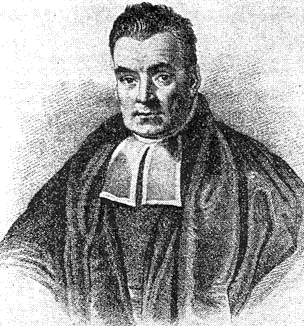
\includegraphics[width=\linewidth]{fig/Thomas_Bayes.png} \\[0.5\baselineskip]
\scriptsize
Source: Wikipedia
\end{figure}
\end{column}
\end{columns}
}

\frame{
\frametitle{Bayes' rule (cont.)}
\[f(\theta \mid \bm{Y}) = \frac{f(\bm{Y} \mid \theta)f(\theta)}{f(\bm{Y})}\]
\begin{itemize}
\item This is really just the definition of conditional densities.
\begin{itemize}
\item The denominator $f(\bm{Y}) \equiv \int f(\bm{Y} \mid \theta)f(\theta)\, d\theta$ makes the posterior density integrate to 1.
\end{itemize}
\item The formula also makes intuitive sense: relative to the prior, we up-weight those values $\theta$ that have a high ``probability'' of generating the observed data $\bm{Y}$, i.e., high likelihood value $f(\bm{Y} \mid \theta)$.
\item The posterior synthesizes two pieces of information: prior knowledge and the new data.
\begin{itemize}
\item Neither piece is infallible: the data has noise (sampling error) and our prior could be wrong. So we should not rely exclusively on either piece.
\end{itemize}
\end{itemize}
}

\frame{
\frametitle{AR(1) example}
\begin{itemize}
\item Let's do an analytical example to see the mechanics of Bayesian inference (though this course will emphasize computation).
\item Consider an AR(1) model with normally distributed shocks:
\[y_t = \rho y_{t-1} + u_t,\quad u_t \overset{iid}{\sim} N(0,\sigma^2).\]
For simplicity, we omit the intercept and assume $\sigma$ is \emph{known}.
\item Prior distribution for the unknown $\rho$:
\[\rho \sim N(m,\lambda^2).\]
\vspace{-\baselineskip}
\begin{itemize}
\item Centered at $\rho=m$. This is our ``best guess'' for $\rho$ \emph{a priori}.
\item Larger $\lambda$ $\Longrightarrow$ more prior uncertainty.
\end{itemize}
\item Prior density:
\[f(\rho) = \frac{1}{\sqrt{2\pi\lambda^2}}e^{-(\rho-m)^2/(2\lambda^2)}.\]
\end{itemize}
}

\frame{
\frametitle{AR(1) example: likelihood function}
\begin{itemize}
\item Next, let's derive the likelihood function for a data set $\bm{Y} \equiv (y_1,y_2,\dots,y_T)'$ of size $T$.
\item By definition of conditional densities,
\[f(y_1,y_2,y_3 \mid \rho) = f(y_3 \mid y_2,y_1,\rho)f(y_2 \mid y_1,\rho)f(y_1 \mid \rho).\]
\item Generalizing:
\[f(\bm{Y} \mid \rho) = f(y_1,\dots,y_T \mid \rho) = f(y_1 \mid \rho)\prod_{t=2}^T f(y_t \mid y_{t-1},y_{t-2},\dots,y_1,\rho).\]
\end{itemize}
}

\frame{
\frametitle{AR(1) example: likelihood function (cont.)}
\begin{itemize}
\item In the Gaussian AR(1) model,
\[(y_t \mid y_{t-1},y_{t-2},\dots,y_1,\rho) \sim N(\rho y_{t-1},\sigma^2),\]
corresponding to the conditional density
\[f(y_t \mid y_{t-1},\rho) = \frac{1}{\sqrt{2\pi\sigma^2}}e^{-(y_t-\rho y_{t-1})^2/(2\sigma^2)}.\]
\item Then the likelihood equals
\begin{align*}
f(\bm{Y} \mid \rho) &= f(y_1 \mid \rho)\prod_{t=2}^T \frac{1}{\sqrt{2\pi\sigma^2}}e^{-(y_t-\rho y_{t-1})^2/(2\sigma^2)} \\
&= f(y_1 \mid \rho)(2\pi\sigma^2)^{-(T-1)/2}e^{\sum_{t=2}^T -(y_t-\rho y_{t-1})^2/(2\sigma^2)}.
\end{align*}
\item It's conventional to ignore the first factor $f(y_1 \mid \rho)$ for tractability.
\end{itemize}
}

\frame{
\frametitle{AR(1) example: posterior}
\begin{itemize}
\item Bayes' rule:
\begin{align*}
f(\rho \mid \bm{Y}) &= \frac{\frac{1}{\sqrt{2\pi\lambda^2}}e^{-(\rho-m)^2/(2\lambda^2)}(2\pi\sigma^2)^{-(T-1)/2}e^{\sum_{t=2}^T -(y_t-\rho y_{t-1})^2/(2\sigma^2)}}{f(\bm{Y})} \\
&= C_1 \times e^{-(\rho-m)^2/(2\lambda^2) -\sum_{t=2}^T (y_t-\rho y_{t-1})^2/(2\sigma^2)} \\
&= C_2 \times e^{-(\rho-\bar{\rho})^2/(2\bar{\tau}^2)},
\end{align*}
where $C_1,C_2$ are constants that don't depend on $\rho$,
\[\bar{\rho} \equiv \frac{\bar{\tau}^2}{\lambda^2} m + \left(1-\frac{\bar{\tau}^2}{\lambda^2}\right)\hat{\rho},\quad \bar{\tau}^2 \equiv \frac{1}{\lambda^{-2} + \sum_{t=2}^T y_{t-1}^2/\sigma^2},\]
and $\hat{\rho} \equiv \sum_{t=2}^T y_ty_{t-1} / \sum_{t=2}^T y_{t-1}^2$ is the usual OLS estimator.
\begin{itemize}
\item \alert{Exercise} (tedious): verify the last step.
\end{itemize}
\end{itemize}
}

\frame{
\frametitle{AR(1) example: posterior (cont.)}
\[f(\rho \mid \bm{Y}) = C_2 \times e^{-(\rho-\bar{\rho})^2/(2\bar{\tau}^2)}\]
\begin{itemize}
\item We recognize this as the density of a normal distribution with mean $\bar{\rho}$ and variance $\bar{\tau}^2$.
\begin{itemize}
\item For the density to integrate to 1, we must have $C_2 = (2\pi \bar{\tau}^2)^{-1/2}$.
\end{itemize}
\item So the posterior distribution for $\rho$ is normal:
\[\boxed{(\rho \mid \bm{Y}) \sim N\left(\bar{\rho},\bar{\tau}^2\right)}.\]
\item The data has caused us to update the prior mean $m$ to the posterior mean $E[\rho \mid \bm{Y}] = \bar{\rho}$, and the prior variance $\lambda^2$ to the posterior variance $\var(\rho \mid \bm{Y}) = \bar{\tau}^2$.
\end{itemize}
}

\frame{
\frametitle{AR(1) example: posterior mean}
\[\bar{\rho} \equiv \frac{\bar{\tau}^2}{\lambda^2} m + \left(1-\frac{\bar{\tau}^2}{\lambda^2}\right)\hat{\rho},\quad \bar{\tau}^2 \equiv \frac{1}{\lambda^{-2} + \sum_{t=2}^T y_{t-1}^2/\sigma^2}\]
\begin{itemize}
\item The posterior mean $E[\rho \mid \bm{Y}] = \bar{\rho}$ is a weighted average of the prior mean $m$ and the OLS estimator $\hat{\rho}$.
\begin{itemize}
\item The Bayesian estimator $\bar{\rho}$ \textbf{shrinks} the frequentist estimator $\hat{\rho}$ toward the prior mean $m$.
\end{itemize}
\item Weight $\bar{\tau}^2/\lambda^2 \in [0,1]$ on prior mean = ratio of the posterior variance to the prior variance of $\rho$.
\item \alert{Exercise:} show that the weight on the prior mean converges to 0 (so $\bar{\rho} \to \hat{\rho}$) if either\dots
\begin{itemize}
\item $\lambda^2 \to \infty$ (the data dominates when our prior is very uncertain/\textbf{diffuse}).
\item $T \to \infty$ (the data dominates the prior in large samples).
\end{itemize}
\end{itemize}
}

\frame{
\centering
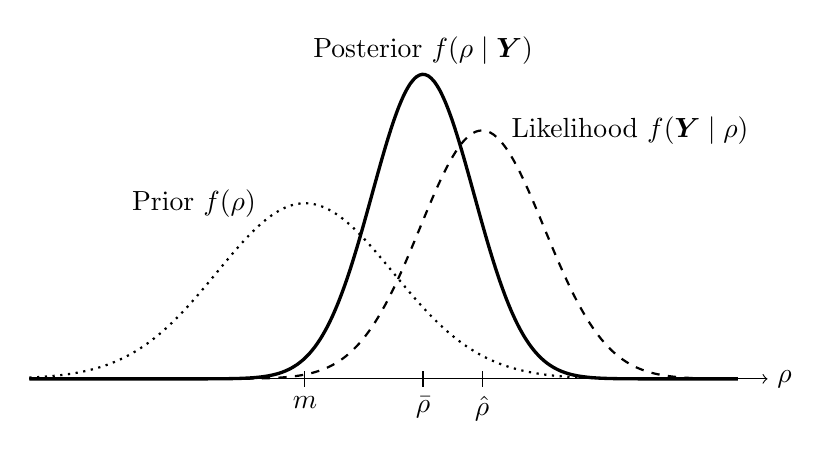
\begin{tikzpicture}[
  scale=2.5,
  prior/.style={thick, dotted, smooth, samples=120},
  likelihood/.style={thick, dashed, smooth, samples=120},
  posterior/.style={very thick, smooth, samples=120}
]
  \def\axL{-1.8}
  \def\axR{1.8}

  \draw[->] (\axL,0) -- (\axR+0.15,0) node[right] {$\rho$};

  % Slide 1: prior (m=-0.4, var=0.20)
  \onslide<1->{%
    \draw[prior, domain=\axL:\axR]
      plot (\x, {0.892*exp(-(\x+0.4)^2/(2*0.20))});
    \draw (-0.4,0.04) -- (-0.4,-0.04) node[below] {$m$};
    \node[anchor=east] at (-0.6,0.892) {Prior $f(\rho)$};
  }

  % Slide 2: + likelihood (rho-hat=0.5, var=0.10)
  \onslide<2->{%
    \draw[likelihood, domain=\axL:\axR]
      plot (\x, {1.262*exp(-(\x-0.5)^2/(2*0.10))});
    \draw (0.5,0.04) -- (0.5,-0.04) node[below] {$\hat{\rho}$};
    \node[anchor=west] at (0.6,1.262) {Likelihood $f(\bm{Y} \mid \rho)$};
  }

  % Slide 3: + posterior (rho-bar=0.2, var=1/15, precision-weighted update)
  \onslide<3->{%
    \draw[posterior, domain=\axL:\axR]
      plot (\x, {1.547*exp(-(\x-0.2)^2/(2*0.067))});
    \draw (0.2,0.04) -- (0.2,-0.04) node[below] {$\bar{\rho}$};
    \node[anchor=south] at (0.2,1.547) {Posterior $f(\rho \mid \bm{Y})$};
  }
\end{tikzpicture}
}

\frame{
\frametitle{AR(1) example: credible interval}
\begin{itemize}
\item Let $Q_\alpha$ be the $\alpha$-quantile of the standard normal distribution.
\item Recall the posterior distribution:
\[(\rho \mid \bm{Y}) \sim N\left(\bar{\rho},\bar{\tau}^2\right).\]
\item Then
\[\boxed{P\left(\rho \in \left[\bar{\rho} - Q_{1-\alpha/2}\bar{\tau},\bar{\rho} + Q_{1-\alpha/2}\bar{\tau}\right] \;\Big|\; \bm{Y}\right) = 1-\alpha}.\]
This interval is called an (equal-tailed) $1-\alpha$ \textbf{credible interval} for $\rho$.
\item A Bayesian can say: the probability that $\rho$ lies in this \emph{particular} interval is $1-\alpha$, given the data that we \emph{actually observed}.
\begin{itemize}
\item Contrasts with the interpretation of a frequentist confidence interval!
\end{itemize}
\end{itemize}
}

\frame{
\frametitle{Summarizing the posterior in general models}
\[f(\theta \mid \bm{Y}) = \frac{f(\bm{Y} \mid \theta)f(\theta)}{f(\bm{Y})}\]
\vspace{-0.5\baselineskip}
\begin{itemize}
\item For some models and priors, the posterior density does not have a simple, known form (e.g., normal).
\item It's typically easy to evaluate the prior density $f(\theta)$ and the likelihood $f(\bm{Y} \mid \theta)$. But the \textbf{marginal density} $f(\bm{Y}) \equiv \int f(\bm{Y} \mid \theta)f(\theta)\,d\theta$ may be intractable.
\item Similarly, it's often intractable to directly evaluate posterior summaries such as the mean
\[E[\theta \mid \bm{Y}] = \int \theta f(\theta \mid \bm{Y})\,d\theta.\]
\item While standard numerical integration could work if $\theta$ has dimension 1 or 2, it won't work in realistic models with many parameters.
\end{itemize}
}

\frame{
\frametitle{Summarizing the posterior in general models (cont.)}
\[f(\theta \mid \bm{Y}) = \frac{f(\bm{Y} \mid \theta)f(\theta)}{f(\bm{Y})}\]
\vspace{-0.5\baselineskip}
\begin{itemize}
\item However, suppose we found a way to randomly \textbf{sample} from the posterior distribution without having to derive it analytically or directly evaluate high-dimensional integrals.
\item If we manage to generate draws $\theta_{(0)},\theta_{(1)},\dots,\theta_{(B)}$ from the posterior distribution on our computer, we can summarize the distribution by computing their sample mean, median, percentiles, etc.
\item For example,
\[E[\theta \mid \bm{Y}] \approx \frac{1}{B+1}\sum_{b=0}^B \theta_{(b)}.\]
\end{itemize}
}

\frame{
\frametitle{MCMC}
\[f(\theta \mid \bm{Y}) = \frac{f(\bm{Y} \mid \theta)f(\theta)}{f(\bm{Y})}\]
\begin{itemize}
\item \textbf{Markov Chain Monte Carlo} (MCMC) methods are designed to randomly sample from the distribution whose density is proportional to the numerator $f(\bm{Y} \mid \theta)f(\theta)$.
\item They do this by stochastically ``walking around'' in the parameter space for $\theta$, tending to prefer steps that increase $f(\bm{Y} \mid \theta)f(\theta)$.
\item But the algorithm also sometimes moves in directions that \emph{decrease} $f(\bm{Y} \mid \theta)f(\theta)$, so as not to get stuck at a single point (which would not explore the full distribution).
\end{itemize}
}

\frame{
\frametitle{MCMC (cont.)}
\begin{itemize}
\item Prototypical MCMC algorithm:
\begin{itemize}
\item Draw an initial parameter vector $\theta_{(0)}$.
\item For each iteration $b=1,\dots,B$:
\smallskip
\begin{enumerate}
\item \textbf{Propose} a new draw $\theta_{(b)}^*$.
\item \textbf{Accept} this draw and set $\theta_{(b)}=\theta_{(b)}^*$ with a probability that's increasing in $f(\bm{Y} \mid \theta)f(\theta)$. Otherwise, \textbf{reject} the draw and stay put: $\theta_{(b)}=\theta_{(b-1)}$.
\end{enumerate}
\end{itemize}
\item This generates a serially correlated time series of draws $\theta_{(0)},\theta_{(1)},\dots,\theta_{(B)}$. Called an MCMC \textbf{chain}.
\item The proposals and acceptance probability are constructed in an ingenious way to ensure that the chain has a stationary distribution whose density is exactly our target posterior density
\[f(\theta \mid \bm{Y}) = \frac{f(\bm{Y} \mid \theta)f(\theta)}{f(\bm{Y})}.\]
\end{itemize}
}

\frame{
\centering
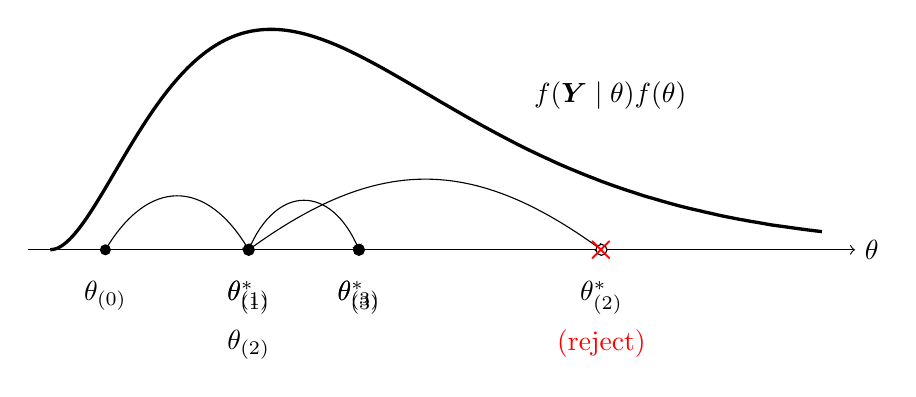
\begin{tikzpicture}[
  xscale=1.4,
  yscale=2.8,
  density/.style={very thick, smooth, samples=120},
  filled/.style={circle, fill=black, minimum size=4pt, inner sep=0},
  open/.style={circle, fill=white, draw=black, minimum size=4pt, inner sep=0}
]
  % x-axis
  \draw[->] (-0.2,0) -- (7.3,0) node[right] {$\theta$};

  % Density: skewed unimodal, mode at theta=2
  \draw[density, domain=0:7]
    plot (\x, {(\x/2)^2 * exp(2-\x)});

  \node[anchor=west] at (4.3,0.7) {$f(\bm{Y} \mid \theta)f(\theta)$};

  % --- Initial: theta_(0) ---
  \onslide<1->{%
    \node[filled] at (0.5,0) {};
    \node[below] at (0.5,-0.10) {$\theta_{(0)}$};
  }

  % --- Step 1: propose theta_(1)^* ---
  \onslide<2>{\draw[->] (0.5,0) to[bend left=40] (1.8,0);}
  \onslide<2->{\node[open] at (1.8,0) {};}
  \onslide<2>{\node[below] at (1.8,-0.10) {$\theta_{(1)}^*$};}

  % --- Step 1: accept (chain at theta_(1)); label persists ---
  \onslide<3->{%
    \node[filled] at (1.8,0) {};
    \node[below] at (1.8,-0.10) {$\theta_{(1)}$};
  }

  % --- Step 2: propose theta_(2)^* (only visible while pending decision) ---
  \onslide<4>{\draw[->] (1.8,0) to[bend left=20] (5,0);}
  \onslide<4-5>{%
    \node[open] at (5,0) {};
    \node[below] at (5,-0.10) {$\theta_{(2)}^*$};
  }

  % --- Step 2: reject (only on slide 5; rejected draw disappears afterwards) ---
  \onslide<5>{%
    \node[red] at (5,0) {\large$\bm{\times}$};
    \node[below, red] at (5,-0.32) {(reject)};
  }

  % --- Chain at theta_(2) = theta_(1) from slide 5 onwards: label stacks below theta_(1) ---
  \onslide<6->{\node[below] at (1.8,-0.32) {$\theta_{(2)}$};}

  % --- Step 3: propose theta_(3)^* ---
  \onslide<7>{\draw[->] (1.8,0) to[bend left=50] (2.8,0);}
  \onslide<7->{\node[open] at (2.8,0) {};}
  \onslide<7>{\node[below] at (2.8,-0.10) {$\theta_{(3)}^*$};}

  % --- Step 3: accept ---
  \onslide<8->{%
    \node[filled] at (2.8,0) {};
    \node[below] at (2.8,-0.10) {$\theta_{(3)}$};
  }

\end{tikzpicture}
\onslide<9->{%
\begin{itemize}
\item Since the algorithm is more likely to accept proposals that increase the (un-normalized) density $f(\bm{Y} \mid \theta)f(\theta)$, most draws will be in the region with high density.
\item But we do sometimes accept proposals with lower density, so we also get draws in the low-density region.
\end{itemize}
}
}

\frame{
\frametitle{MCMC (cont.)}
\begin{itemize}
\item The distribution of the draws in the chain eventually \textbf{converges} to the stationary distribution (i.e., the posterior distribution) as $B \to \infty$.
\item However, if the initial parameter $\theta_{(0)}$ is far from the center of the stationary distribution, it may take many iterations to converge.
\begin{itemize}
\item This is just like how a stationary AR(1) process depends on the initial value $y_0$ at first, but as time goes on, the effect of the initial value vanishes.
\end{itemize}
\item So in practice we discard the first several steps from the MCMC chain. The discarded draws are called \textbf{burn-in}.
\item After burn-in, the chain ought to look stationary.
\end{itemize}
}

\frame{
\frametitle{Stan}
\begin{itemize}
\item Designing efficient MCMC procedures is hard and very technical work.
\item The Bayesian software \textbf{Stan} automates this process.
\begin{itemize}
\item Uses a variant of MCMC called ``Hamiltonian Monte Carlo'' (HMC).
\item Can be called from several programming languages, such as Python, R, Matlab, and Julia.
\item The documentation is well-written, with many examples.
\end{itemize}
\item Researchers just need to supply a ``model file'' specifying the prior and likelihood function in natural mathematical notation.
\item Then Stan figures out how to do MCMC sampling on its own.
\item After sampling, Stan generates posterior summaries and diagnostics.
\end{itemize}
}

\frame{
\frametitle{Bayesian estimation of an AR($p$) model}
\begin{itemize}
\item We'll apply Stan to an AR($p$) model with normally distributed shocks:
\[y_t = c + a_1y_{t-1} + \dots + a_p y_{t-p} + u_t,\quad u_t \overset{iid}{\sim} N(0,\sigma^2).\]
\item We would like to estimate this with Bayesian methods.
\begin{itemize}
\item This particular model is actually not hard to analyze analytically, but Stan can be useful also in more difficult models, as we'll see.
\end{itemize}
\item Data set: $\bm{Y} \equiv (y_1,y_2,\dots,y_T)'$.
\item Parameter vector: $\bm{\theta} \equiv (c,a_1,\dots,a_p,\sigma)'$. Dimension $(p+2) \times 1$.
\end{itemize}
}

\frame{
\frametitle{Bayesian AR($p$): likelihood}
\begin{itemize}
\item In this model,
\[(y_t \mid y_{t-1},y_{t-2},\dots,y_1,\bm{\theta}) \sim N(c + \bm{x}_t'\bm{\beta},\sigma^2),\]
\[\text{where}\quad \bm{x}_t \equiv \underbrace{(y_{t-1},\dots,y_{t-p})'}_{p \times 1},\quad \bm{\beta} \equiv \underbrace{(a_1,a_2,\dots,a_p)'}_{p \times 1}.\]
\item Similar to the AR(1) case,
\begin{align*}
f(\bm{Y} \mid \bm{\theta}) &= f(y_1,\dots,y_p \mid \bm{\theta})\prod_{t=p+1}^T f(y_t \mid y_{t-1},y_{t-2},\dots,y_1,\bm{\theta}) \\
&= f(y_1,\dots,y_p \mid \bm{\theta}) (2\pi \sigma^2)^{-(T-p)/2} e^{-\sum_{t=p+1}^T (y_t - c - \bm{x}_t'\bm{\beta})^2/(2\sigma^2)}.
\end{align*}
\item It's conventional to ignore the first factor $f(y_1,\dots,y_p \mid \bm{\theta})$.
\end{itemize}
}

\frame{
\frametitle{Bayesian AR($p$): likelihood (cont.)}
\[f(\bm{Y} \mid \bm{\theta}) = (2\pi \sigma^2)^{-(T-p)/2} e^{-\sum_{t=p+1}^T (y_t - c - \bm{x}_t'\bm{\beta})^2/(2\sigma^2)}\]
\vspace{-0.5\baselineskip}
\begin{itemize}
\item This likelihood function corresponds to the density of the $(T-p) \times 1$ normal random vector $\tilde{\bm{Y}} \equiv (y_{p+1},\dots,y_T)'$:
\[\tilde{\bm{Y}} \sim N\left(c \bm{1} + \bm{X}\bm{\beta},\sigma^2 \bm{I}\right),\]
where $\bm{I}$ is the $(T-p) \times (T-p)$ identity matrix, $\bm{1}$ is a $(T-p) \times 1$ vector of 1's, and
\[\bm{X} \equiv \underbrace{\begin{pmatrix}
\bm{x}_{p+1}, \bm{x}_{p+2}, \dots, \bm{x}_T
\end{pmatrix}'}_{(T-p) \times p}.\]
\item We exploit this in the Stan model file below.
\end{itemize}
}

\frame{
\frametitle{Bayesian AR($p$): prior}
\begin{itemize}
\item Often when forecasting macro time series, it's surprisingly hard to beat the naive no-change forecast: $y_{t+1|t}=y_t$.
\item In the AR($p$) model, the no-change forecast is optimal for the parameters $a_1=1$ and $a_\ell =0$ for $\ell \geq 2$, yielding the random walk
\[y_t = y_{t-1} + u_t.\]
\item This suggests a prior distribution where
\[E[a_1]=1,\quad E[a_2]=E[a_3]=\dots=E[a_p]=0.\]
\end{itemize}
}

\frame{
\frametitle{Bayesian AR($p$): prior (cont.)}
\begin{itemize}
\item The \textbf{Minnesota prior} (invented by researchers at University of Minnesota) specifies
\[a_\ell \sim N\left(m_\ell, \frac{\lambda^2}{\ell^2} \right),\quad \text{where}\quad m_1 \equiv 1,\quad m_2=\dots=m_p=0.\]
\item ``Shrinks'' the coefficient $a_1$ towards 1 and $a_2,\dots,a_p$ towards 0.
\item More shrinkage (due to smaller prior variance) at longer lags $\ell$.
\begin{itemize}
\item Effectively reduces the dimension of the parameter space. So we can use a large lag order $p$ without overfitting.
\item For large $\ell$, $|\hat{a}_\ell|$ must be very large to shift the posterior away from 0.
\end{itemize}
\item $\lambda^2$ governs the overall degree of shrinkage.
\begin{itemize}
\item Common choice in literature: $\lambda=0.2$.
\end{itemize}
\end{itemize}
}

\frame{
\centering
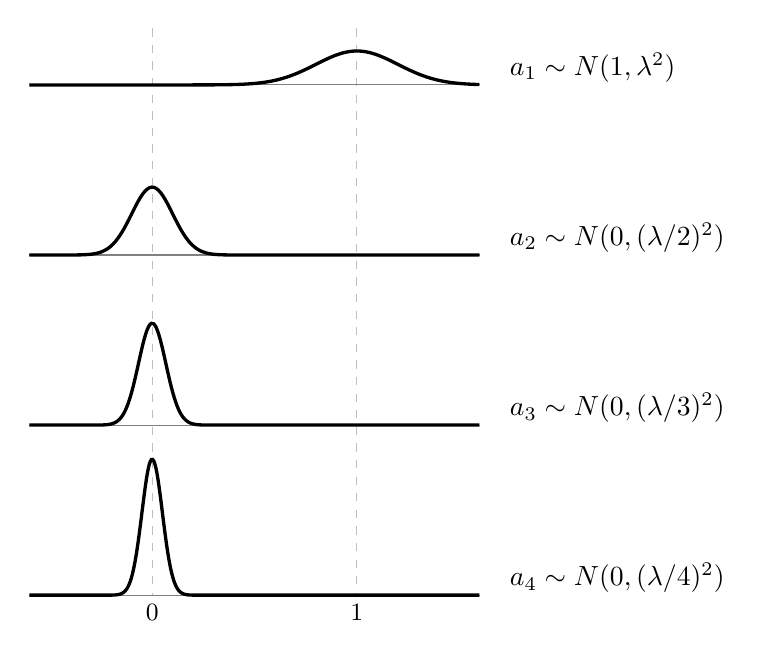
\begin{tikzpicture}[
  xscale=2.6,
  yscale=1.2,
  curve/.style={very thick, smooth, samples=200},
  ax/.style={gray},
  ref/.style={dashed, lightgray}
]
  \def\axL{-0.6}
  \def\axR{1.6}

  % shrinkage targets: faint vertical lines at a_l = 0 and a_l = 1
  \draw[ref] (0,0.6) -- (0,-5.4);
  \draw[ref] (1,0.6) -- (1,-5.4);

  % l = 1:  N(1, lambda^2),  sd = 0.2
  \draw[ax] (\axL,0) -- (\axR,0);
  \draw[curve, domain=\axL:\axR] plot (\x, {0.359*exp(-(\x-1)^2/(2*0.04))});
  \node[anchor=west] at (\axR+0.1,0.18) {$a_1 \sim N(1,\lambda^2)$};

  % l = 2:  N(0, lambda^2/4),  sd = 0.1
  \draw[ax] (\axL,-1.8) -- (\axR,-1.8);
  \draw[curve, domain=\axL:\axR] plot (\x, {-1.8 + 0.718*exp(-(\x)^2/(2*0.01))});
  \node[anchor=west] at (\axR+0.1,-1.8+0.18) {$a_2 \sim N(0,(\lambda/2)^2)$};

  % l = 3:  N(0, lambda^2/9),  sd = 0.067
  \draw[ax] (\axL,-3.6) -- (\axR,-3.6);
  \draw[curve, domain=\axL:\axR] plot (\x, {-3.6 + 1.077*exp(-(\x)^2/(2*0.004444))});
  \node[anchor=west] at (\axR+0.1,-3.6+0.18) {$a_3 \sim N(0,(\lambda/3)^2)$};

  % l = 4:  N(0, lambda^2/16),  sd = 0.05
  \draw[ax] (\axL,-5.4) -- (\axR,-5.4);
  \draw[curve, domain=\axL:\axR] plot (\x, {-5.4 + 1.436*exp(-(\x)^2/(2*0.0025))});
  \node[anchor=west] at (\axR+0.1,-5.4+0.18) {$a_4 \sim N(0,(\lambda/4)^2)$};

  % shared axis labels (the two shrinkage targets)
  \node[below] at (0,-5.4) {\small $0$};
  \node[below] at (1,-5.4) {\small $1$};
\end{tikzpicture}
}

\frame{
\frametitle{Bayesian AR($p$): prior (cont.)}
\begin{itemize}
\item For the intercept and the shock standard deviation it's common to use very diffuse priors, such as
\[c \sim N\left(0,10^4 \hat{\sigma}_y^2\right),\]
\[\sigma \sim \text{Cauchy}_+(0, \hat{\sigma}_y),\]
where $\hat{\sigma}_y^2$ is the sample variance of $\lbrace y_t \rbrace$.
\begin{itemize}
\item ``$\text{Cauchy}_+$'' is a Cauchy distribution restricted to the positive real line (a very fat-tailed distribution).
\end{itemize}
\item Finally, we assume all $p+2$ parameters in $\bm{\theta}$ are independent \emph{a priori}: their joint prior density is the product of the marginal densities.
\item We now have the likelihood and the prior. Let's crank up Stan!
\end{itemize}
}

\frame{
\begin{figure}
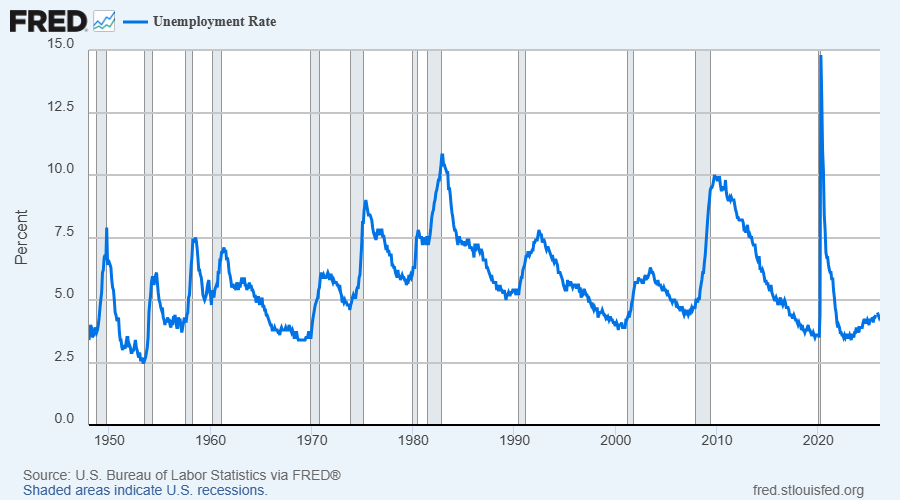
\includegraphics[width=\linewidth]{fig/fred_unrate.png} \\
\bigskip
Discard data from 2020 onwards (we'll discuss how to model the massive Covid shock in the next slide deck)
\end{figure}
}

\begin{frame}[fragile]
My Stan model file \texttt{slides12\_ar.stan}:
\bigskip
\scriptsize
\begin{verbatim}
data {
  int<lower=1> T;              // effective sample size
  int<lower=1> p;              // lag order
  vector[T] y;                 // observed series
  matrix[T, p] X;              // lag matrix
  real<lower=0> lambda;        // prior tightness
  real<lower=0> scale_sigma;   // prior scale for sigma
  real<lower=0> scale_c;       // prior scale for intercept c
}

parameters {
  real c;                      // intercept
  vector[p] a;                 // AR coefficients
  real<lower=0> sigma;         // innovation std. dev.
}
\end{verbatim}
\normalsize
(continued next slide)
\end{frame}

\begin{frame}[fragile]
\scriptsize
\begin{verbatim}
model {
  // Minnesota prior on AR coefficients
  for (l in 1:p) {
    real m_ = (l == 1) ? 1.0 : 0.0;
    real sd_ = lambda / l;
    a[l] ~ normal(m_, sd_);
  }

  // Intercept prior
  c ~ normal(0, scale_c);

  // Innovation std. dev.
  sigma ~ cauchy(0, scale_sigma);

  // Likelihood (vectorized)
  y ~ normal(c + X * a, sigma);
}
\end{verbatim}
\bigskip
\normalsize
Note: Stan (like \texttt{scipy}) parametrizes $N(0,\sigma)$ instead of $N(0,\sigma^2)$.
\end{frame}

\begin{frame}[fragile]
\scriptsize
\begin{verbatim}
p = 12 # lag length
X = sm.tsa.tsatools.lagmat(y_full, maxlag=p, trim='both') # lag matrix

# Data for Stan
std_y = y_full.std()
stan_data = {
    'T': X.shape[0],
    'p': p,
    'y': y_full[p:],
    'X': X,
    'lambda': 0.2,
    'scale_sigma': std_y,
    'scale_c': 100*std_y,
}

# Compile and sample
model = CmdStanModel(stan_file='slides12_ar.stan')
fit = model.sample(data=stan_data, seed=31150, chains=4,
                   iter_warmup=1000, iter_sampling=1000, show_progress=True)

print(fit.summary())
\end{verbatim}
\end{frame}

\frame{
\begin{figure}
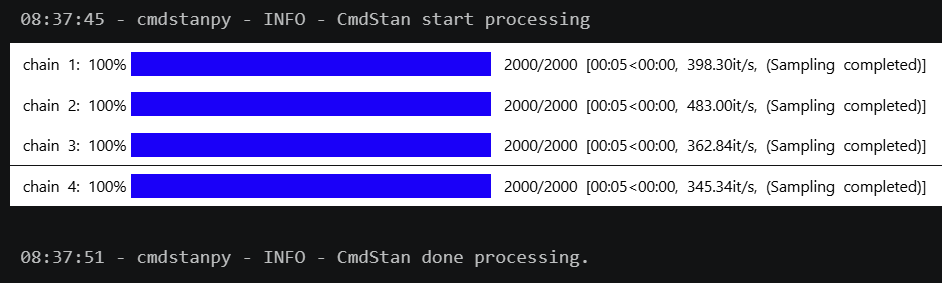
\includegraphics[width=\linewidth]{fig/stan_sampling.png}
\end{figure}
\begin{itemize}
\item First Stan compiles the sampling program (only done once).
\item Then runs 4 chains in parallel from randomly drawn initial values.
\item For each chain: 1000 burn-in draws discarded, then last 1000 draws retained.
\item Here sampling is very fast (5 seconds). Can take much longer in more complicated models.
\end{itemize}
}

\begin{frame}[fragile]
\scriptsize
\begin{verbatim}
              Mean      MCSE    StdDev       MAD           5%          50%  \
lp__   1010.280000  0.063370  2.759430  2.557710  1005.270000  1010.630000   
c         0.089636  0.000391  0.025454  0.025671     0.047837     0.089861   
a[1]      1.012370  0.000595  0.032229  0.032269     0.960301     1.011730   
a[2]      0.172059  0.000791  0.042703  0.042244     0.099819     0.172488   
a[3]     -0.045320  0.000651  0.037394  0.037117    -0.106699    -0.044841   
[...]
a[12]     0.002350  0.000201  0.012718  0.012585    -0.018468     0.002253   
sigma     0.192057  0.000074  0.004798  0.004618     0.184378     0.191976   

               95%  ESS_bulk  ESS_tail  ESS_bulk/s     R_hat  
lp__   1014.130000   1952.88   2720.81     169.344  1.000220  
c         0.131474   4250.83   3084.38     368.612  1.000550  
a[1]      1.065190   2965.11   2705.60     257.120  1.003520  
a[2]      0.240726   2952.46   2658.34     256.024  1.000210  
a[3]      0.015843   3348.71   2931.60     290.384  1.001960  
[...]
a[12]     0.023426   4044.95   3335.40     350.758  1.000380  
sigma     0.200040   4248.17   3160.73     368.381  1.001310
\end{verbatim}
\bigskip
\normalsize
Note: parameters $a_4,a_5,\dots,a_{11}$ omitted from output for legibility.
\begin{tikzpicture}[overlay, remember picture]
  \only<2>{%
    \circleoverlay[cx=-3.75cm, cy=2.8cm, r=0.7cm,
                   tx=0cm, ty=-1cm, text anchor=north]{Posterior mean \\ $E[a_1 \mid \bm{Y}]$}%
  }
  \only<3>{%
    \circleoverlay[cx=-0.78cm, cy=2.8cm, r=0.7cm,
                   tx=0cm, ty=-1cm, text anchor=north]{Posterior std.\ dev. \\ $\sqrt{\var(a_1 \mid \bm{Y})}$}%
  }
  \only<4>{%
    \circleoverlay[cx=2.67cm, cy=2.8cm, r=0.7cm,
                   tx=0cm, ty=-1cm, text anchor=north]{Posterior 5th \\ percentile of $a_1$}%
  }
  \only<5>{%
    \circleoverlay[cx=4.6cm, cy=2.8cm, r=0.7cm,
                   tx=0cm, ty=-1cm, text anchor=north]{Posterior median \\ $\text{median}(a_1 \mid \bm{Y})$}%
  }
  \only<6>{%
    \circleoverlay[cx=-3.75cm, cy=-0.5cm, r=0.7cm,
                   tx=0cm, ty=-1cm, text anchor=north]{Posterior 95th \\ percentile of $a_1$}%
  }
\end{tikzpicture}%
\end{frame}

\frame{
\begin{figure}
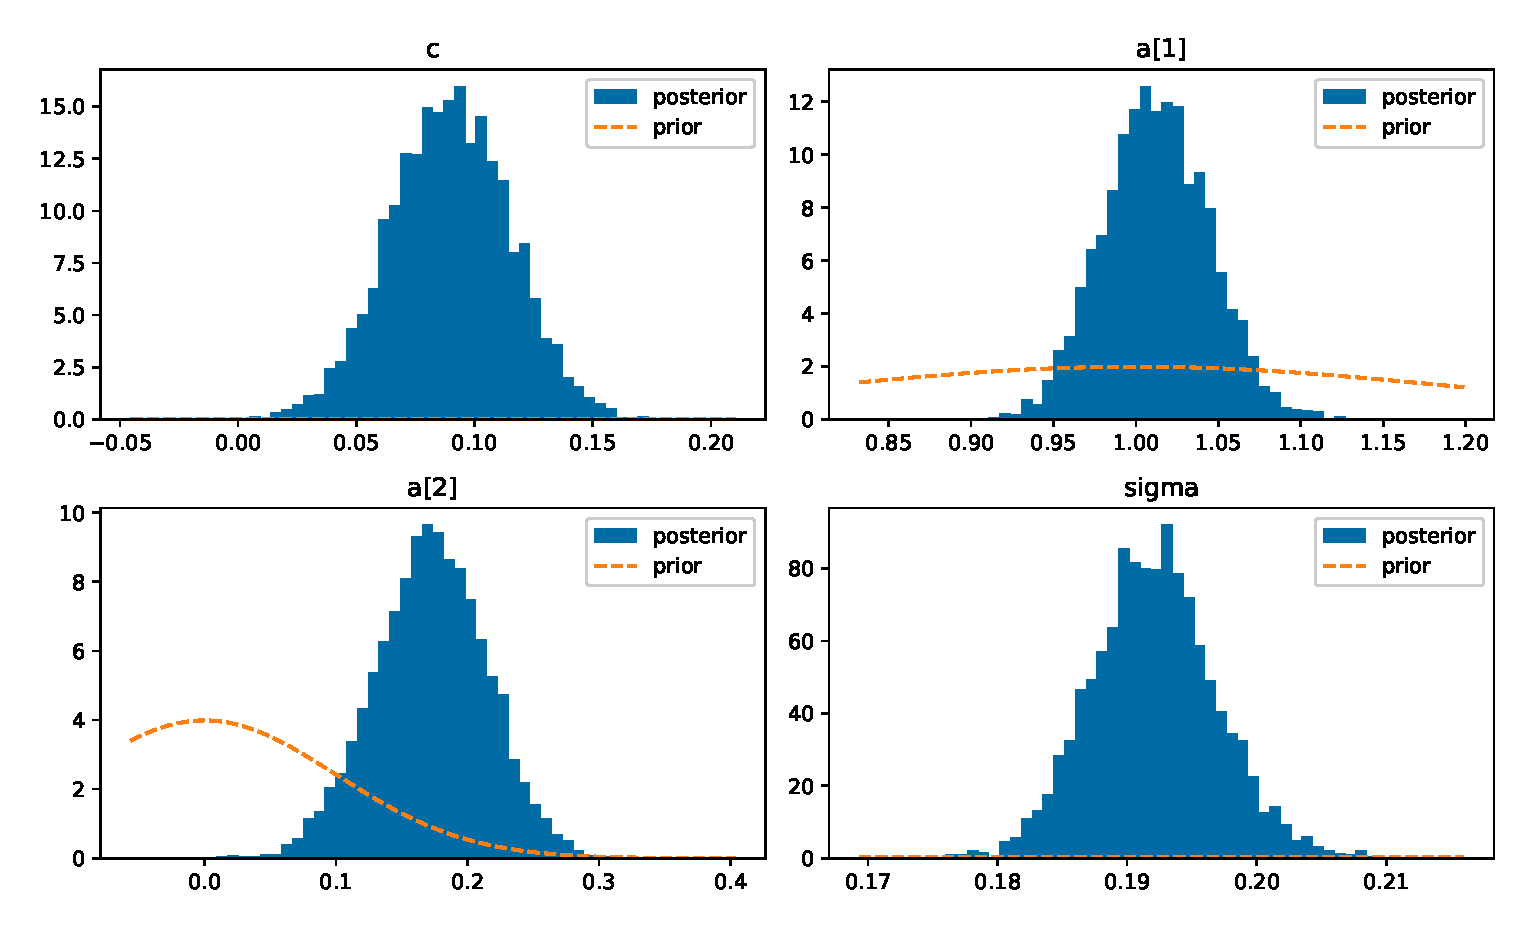
\includegraphics[width=\linewidth]{fig/bayes_ar_posterior.eps} \\
\bigskip
Note: prior densities for $c$ and $\sigma$ are so diffuse that they're barely visible.
\end{figure}
}

\begin{frame}[fragile]
\scriptsize
\begin{verbatim}
# Posterior quantiles
print(np.quantile(draws['a[1]'].values, [0.025, 0.05, 0.95, 0.975]))
\end{verbatim}
\bigskip
\normalsize
\textbf{Result:}
\scriptsize
\begin{verbatim}
[0.95111886 0.96030143 1.06518581 1.07486885]
\end{verbatim}
\bigskip
\normalsize
\begin{itemize}
\item 90\% credible interval for $a_1$: $[0.960,1.065]$
\item 95\% credible interval for $a_1$: $[0.951,1.075]$
\end{itemize}
\end{frame}

\frame{
\frametitle{Convergence diagnostics}
\begin{itemize}
\item It's important to check that the MCMC chain has reached a stationary distribution, after discarding the burn-in.
\item Convergence may fail if the posterior density has multiple peaks or is very non-smooth in some directions.
\item Plot the chains of each individual parameter (called a \textbf{trace plot}) and inspect whether the time series look (i) stationary and (ii) similar across parallel chains.
\end{itemize}
}

\frame{
\begin{figure}
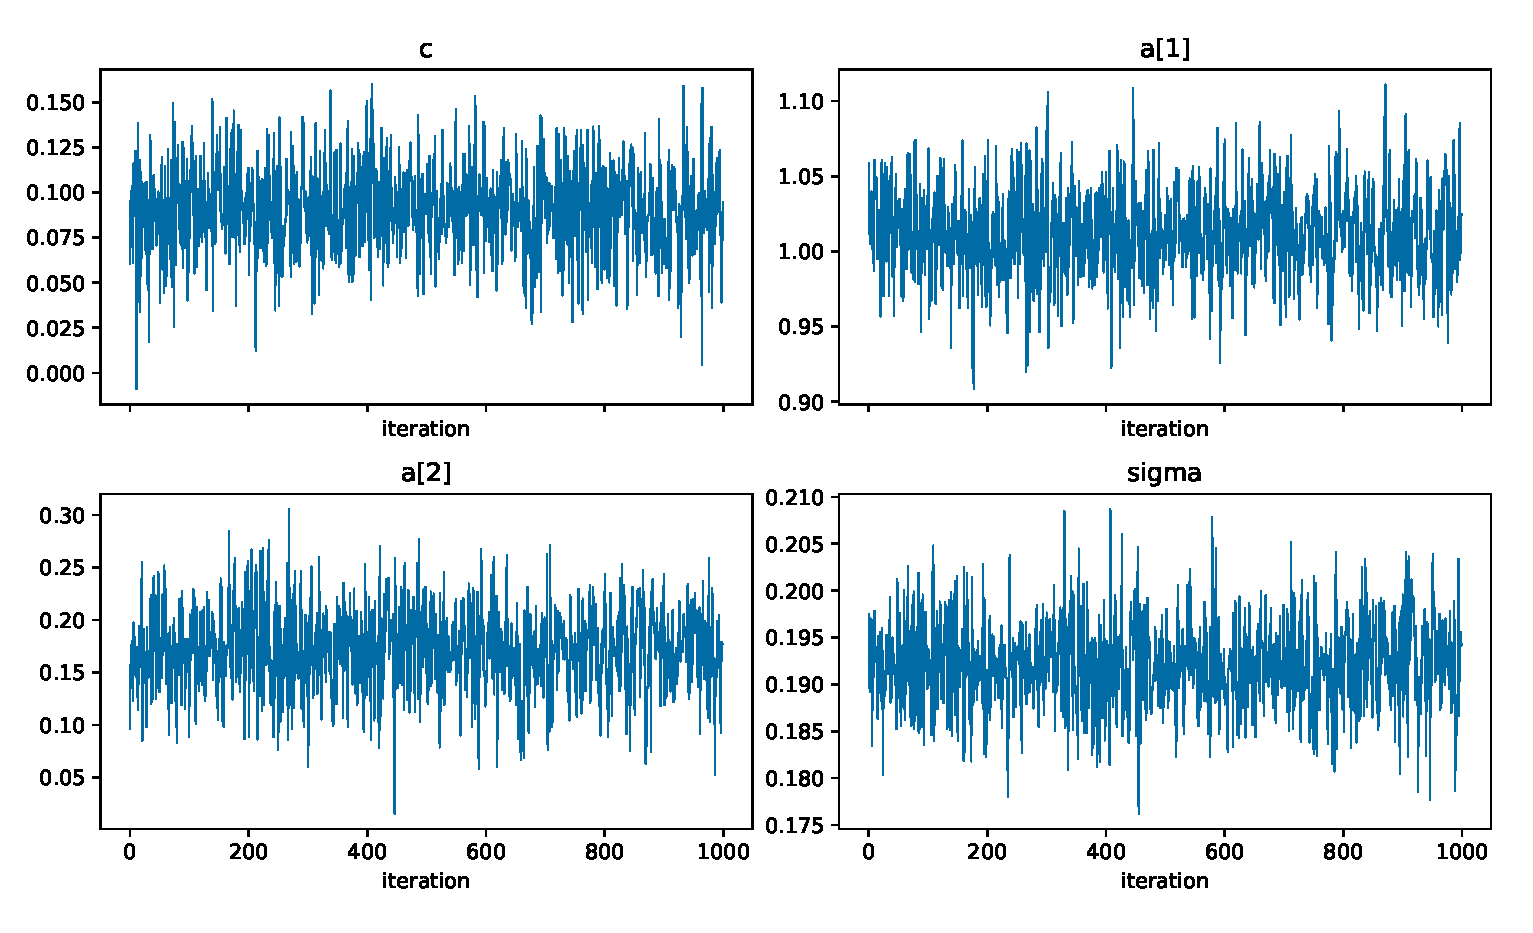
\includegraphics[width=\linewidth]{fig/bayes_ar_trace.eps} \\
\bigskip
Plot of a single chain (out of 4 parallel ones) after burn-in
\end{figure}
}

\frame{
\frametitle{Convergence diagnostics (cont.)}
\begin{itemize}
\item Stan's \texttt{R\_hat} measures how different results are across parallel chains. Ideally, \texttt{R\_hat} $<1.01$.
\item Each chain is serially correlated by design. If the dependence is very high, we need very many draws to accurately approximate posterior means, etc.
\item Stan's \texttt{ESS\_bulk} measures the ``effective sample size'', i.e., the number of draws that are approximately uncorrelated (adjusting for the long-run variance of the chain). Should be in the 1000s.
\end{itemize}
}

\begin{frame}[fragile]
\scriptsize
\begin{verbatim}
              Mean      MCSE    StdDev       MAD           5%          50%  \
lp__   1010.280000  0.063370  2.759430  2.557710  1005.270000  1010.630000   
c         0.089636  0.000391  0.025454  0.025671     0.047837     0.089861   
a[1]      1.012370  0.000595  0.032229  0.032269     0.960301     1.011730   
a[2]      0.172059  0.000791  0.042703  0.042244     0.099819     0.172488   
a[3]     -0.045320  0.000651  0.037394  0.037117    -0.106699    -0.044841   
[...]
a[12]     0.002350  0.000201  0.012718  0.012585    -0.018468     0.002253   
sigma     0.192057  0.000074  0.004798  0.004618     0.184378     0.191976   

               95%  ESS_bulk  ESS_tail  ESS_bulk/s     R_hat  
lp__   1014.130000   1952.88   2720.81     169.344  1.000220  
c         0.131474   4250.83   3084.38     368.612  1.000550  
a[1]      1.065190   2965.11   2705.60     257.120  1.003520  
a[2]      0.240726   2952.46   2658.34     256.024  1.000210  
a[3]      0.015843   3348.71   2931.60     290.384  1.001960  
[...]
a[12]     0.023426   4044.95   3335.40     350.758  1.000380  
sigma     0.200040   4248.17   3160.73     368.381  1.001310
\end{verbatim}
\begin{tikzpicture}[overlay, remember picture]
  \only<2>{%
    \circleoverlay[cx=2.55cm, cy=-0.7cm, r=0.7cm,
                   tx=0.7cm, ty=-0.7cm, text anchor=west]{Good!}%
  }
  \only<3>{%
    \circleoverlay[cx=-2.22cm, cy=-0.7cm, r=0.7cm,
                   tx=0.7cm, ty=-0.7cm, text anchor=west]{Good!}%
  }
\end{tikzpicture}%
\end{frame}

\frame{
\frametitle{Convergence diagnostics (cont.)}
\begin{itemize}
\item If you call \texttt{fit.diagnose()}, Stan performs some automatic convergence diagnostics (but you should also inspect yourself).
\item How to think about and address convergence issues: \\ {\small \url{https://mc-stan.org/learn-stan/diagnostics-warnings.html} }
\end{itemize}
}

\frame{
\frametitle{What did we learn?}
\begin{itemize}
\item Bayesian inference
\begin{itemize}
\item Prior, likelihood, posterior
\item Credible interval
\end{itemize}
\item MCMC
\item Modeling and posterior sampling with Stan
\begin{itemize}
\item Convergence diagnostics
\end{itemize}
\end{itemize}
}

\frame{
\frametitle{Looking ahead}
\begin{itemize}
\item Bayesian forecasting
\item Bayesian (S)VARs
\item Modeling time-varying shock volatility
\item How to handle the massive Covid shock in economic data?
\end{itemize}
}

\end{document}
